\documentclass[12pt,letterpaper,titlepage]{report}

% packages

\usepackage[utf8]{inputenc}
\usepackage{mathptmx}
\usepackage{geometry}
\usepackage{float}
\usepackage{subcaption}
\usepackage{multirow}
\usepackage{makecell}
\usepackage{circuitikz}
\usepackage{pgfplots}

% commands

\newcommand{\myTitle}{Series and Parallel Circuits}
\newcommand{\myName}{Shawn Lutch}
\newcommand{\myPeriod}{PHYS 2240.502}
\pgfplotsset{compat=1.10}

% shamelessly copied and pasted from https://tex.stackexchange.com/a/229158

\ctikzset{bipoles/ammeter/text rotate/.initial=0,
rotation/.style={bipoles/ammeter/text rotate=#1}}

% code from pgfcircbipoles.sty

\makeatletter
\pgfcircdeclarebipole{}{\ctikzvalof{bipoles/ammeter/height}}{ammeter}{\ctikzvalof{bipoles/ammeter/height}}{\ctikzvalof{bipoles/ammeter/width}}{
    \def\pgf@circ@temp{right}
    \ifx\tikz@res@label@pos\pgf@circ@temp
        \pgf@circ@res@step=-1.2\pgf@circ@res@up
    \else
        \def\pgf@circ@temp{below}
        \ifx\tikz@res@label@pos\pgf@circ@temp
            \pgf@circ@res@step=-1.2\pgf@circ@res@up
        \else
            \pgf@circ@res@step=1.2\pgf@circ@res@up
        \fi
    \fi

    \pgfpathmoveto{\pgfpoint{\pgf@circ@res@left}{\pgf@circ@res@zero}}       
    \pgfpointorigin \pgf@circ@res@other =  \pgf@x  \advance \pgf@circ@res@other by -\pgf@circ@res@up
    \pgfpathlineto{\pgfpoint{\pgf@circ@res@other}{\pgf@circ@res@zero}}
    \pgfusepath{draw}

    \pgfsetlinewidth{\pgfkeysvalueof{/tikz/circuitikz/bipoles/thickness}\pgfstartlinewidth}

        \pgfscope
            \pgfpathcircle{\pgfpointorigin}{.9\pgf@circ@res@up}
            \pgfusepath{draw}       
        \endpgfscope    

    \pgftransformrotate{\ctikzvalof{bipoles/ammeter/text rotate}}% <= magic line
    \pgfsetlinewidth{\pgfstartlinewidth}

    \pgfsetarrowsend{latex}
    \pgfpathmoveto{\pgfpoint{\pgf@circ@res@other}{\pgf@circ@res@down}}
    \pgfpathlineto{\pgfpoint{-\pgf@circ@res@other}{\pgf@circ@res@up}}
    \pgfusepath{draw}
    \pgfsetarrowsend{}


    \pgfpathmoveto{\pgfpoint{-\pgf@circ@res@other}{\pgf@circ@res@zero}}
    \pgfpathlineto{\pgfpoint{\pgf@circ@res@right}{\pgf@circ@res@zero}}
    \pgfusepath{draw}


    \pgfnode{circle}{center}{\textbf{A}}{}{}
}
\makeatother % allow rotation of elements in circuit diagram

% metadata

\usepackage[pdftex,
            pdfauthor={\myName{}},
            pdftitle={\myTitle{}},
            pdfsubject={\myPeriod{}},
            pdfproducer={\myName{} via LaTeX},
            pdfcreator={pdflatex}]{hyperref}
			
% layout

\pagenumbering{gobble}
\raggedright
\geometry{
	letterpaper,
	lmargin=0.75in,
	rmargin=0.75in,
	tmargin=1.0in,
	bmargin=1.0in
}

% document

\begin{document}


%% title page


\title{\myTitle{}}
\author{\myName{}\\ \myPeriod{}}
\date{\today}
\maketitle


%% abstract


\section*{Abstract}

TODO


%% introduction

\bigskip
\section*{Introduction}

We use Ohm's Law to describe the relationship between the voltage $V$, current $I$, and equivalent resistance $R_{eq}$ in a circuit:

$$V_{total} = I_{total} \times R_{eq}$$

Using an ammeter and a fixed voltage source, we are able to rearrange Ohm's Law in order to calculate the equivalent resistance of the circuit:

$$R_{eq} = \frac{ V_{total} }{ I_{total} }$$

In this lab, we demonstrate the ability to simplify complex circuits and calculate the $R_{eq}$ with known values for $V$ and $I$.




%% apparatus

\bigskip
\section*{Apparatus}

\begin{itemize}
	\item PASCO Capstone (data acquisition, display, analysis software)
	\item 850 Universal Interface
	\item AC/DC Electronics Laboratory
	\item Patch cords (x8)
	\item Resistors (x6)
		\begin{itemize}
			\item 100 $\Omega$ (brown-black-brown-gold) resistors (x2)
			\item 330 $\Omega$ (orange-orange-brown-gold) resistors (x2)
			\item 560 $\Omega$ (green-blue-brown-gold) resistors (x2)
		\end{itemize}
\end{itemize}


%% procedure

\bigskip
\section*{Procedure}

Given that the resistors in the circuit diagrams are labeled $R_{1\ldots6}$, we first separated and labeled the resistors as instructed by the lab manual:

\bigskip
\begin{minipage}{\linewidth}
\centering
\begin{tabular}{ | c | c | c | c | c | c | }
	\hline
	$R_1$ & $R_2$ & $R_3$ & $R_4$ & $R_5$ & $R_6$ \\
	\hline
	330 $\Omega$ & 560 $\Omega$ & 100 $\Omega$ & 100 $\Omega$ & 560 $\Omega$ & 330 $\Omega$ \\
	\hline
\end{tabular}
\end{minipage}
\bigskip

The precision of each resistor is $\pm 5 \%$, as indicated by the gold band on each. In order to ensure the highest level of accuracy possible in our calculations for the equivalent resistance ($R_{eq}$) of each circuit, we first needed to find the actual resistance of our six resistors, as shown in Table 1. These numbers would be used later in our calculations for the theoretical $R_{eq}$ of each circuit. The following circuit was used to calibrate each resistor $R_n$ by using PASCO Capstone to record the actual resistance to a precision of around $\pm 1 \%$:

\bigskip
\begin{minipage}{\linewidth}
\centering
\begin{circuitikz}
\draw
(2,2) to[battery,l=850 Interface] (2,0)
      to[ammeter,rotation=180] (0,0)
      to[resistor,l=$R_n$] (0,2) -- (2,2)
;
\end{circuitikz}
\end{minipage}
\bigskip



%% data

\bigskip
\section*{Data}


% resistor calibration
\begin{minipage}{\linewidth}
\centering
\captionof{table}{Measured Resistance Values}
\begin{tabular}{ | c | c | c | c | c | c | } \hline

    \thead{$R_n$} & \thead{Ideal \\ $R$ ($\Omega$)} & \thead{Measured \\ $R$ ($\Omega$)} \\ \hline
    $R_1$ & 330 & 315  \\ \hline
    $R_2$ & 560 & 535  \\ \hline
    $R_3$ & 100 & 95.7 \\ \hline
    $R_4$ & 100 & 96.8 \\ \hline
    $R_5$ & 560 & 537  \\ \hline
    $R_6$ & 330 & 314  \\ \hline
    
\end{tabular}
\end{minipage}

\bigskip
\bigskip

% ammeter calibration
\begin{minipage}{\linewidth}
\centering
\captionof{table}{Ammeter Calibration Data}
\begin{tabular}{ | c | c | c | c | } \hline
	\thead{Voltage (V)} & \thead{Theoretical \\ Current (mA)} & \thead{Measured \\ Current (mA)} & \thead{Correction \\ (mA)} \\ \hline
	0 V & 0 mA & 0.3 mA & -0.3 mA \\ \hline
	1 V & 10.3 mA & 10.6 mA & -0.3 mA \\ \hline
	2 V & 20.7 mA & 20.9 mA & 0.2 mA \\ \hline
	3 V & 31.0 mA & 31.0 mA & 0.0 mA \\ \hline
	4 V & 41.3 mA & 41.3 mA & 0.0 mA \\ \hline
	5 V & 51.7 mA & 51.6 mA & 0.1 mA \\ \hline
	6 V & 62.0 mA & 62.1 mA & -0.1 mA \\ \hline
	7 V & 72.3 mA & 72.5 mA & -0.2 mA \\ \hline
\end{tabular}
\end{minipage}

\bigskip
\bigskip

\begin{minipage}{\linewidth}
\centering
\captionof{table}{Measured and Corrected Current}
\begin{tabular}{ | c | c | c | c | } \hline
     \thead{Circuit} & \thead{Theoretical \\ $R_{eq}$ ($\Omega$)} & \thead{Measured \\ Current (A)} & \thead{Corrected \\ Current (A)} \\ \hline
\end{tabular}
\end{minipage}


%% calcs and graphs

\bigskip
\section*{Calculations and Graphs}

\begin{minipage}{\linewidth}
\centering
\captionof{table}{Calculated Resistances}
\begin{tabular}{| c | c | c | c |} \hline
    
    \thead{Circuit} & \thead{Theor. \\ $R_{eq}$ ($\Omega$)} & \thead{Exper. \\ $R_{eq}$ ($\Omega$)} & \thead{\% \\ Diff.} \\ \hline
    
    1 & 850   & 765   & 10.48 \\ \hline
    2 & 198.3 & 193.3 & 2.55  \\ \hline
    3 & 294.0 & 283.0 & 3.81  \\ \hline
    4 & 366.4 & 350.5 & 4.42  \\ \hline
    
    
\end{tabular}
\end{minipage}

\bigskip
\bigskip

\begin{minipage}{\linewidth}
\centering
\captionof{figure}{Resistance of Each Circuit}
<<<<<<< HEAD
=======
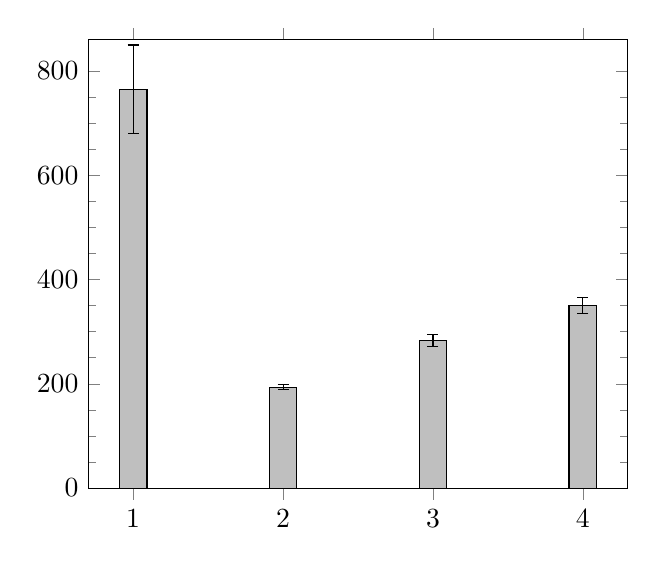
\begin{tikzpicture}

    \begin{axis}[
        xtick = { 1,...,4 },
        xticklabels = { 1, 2, 3, 4 },
        ymax = 860,
        ymin = 0,
        minor y tick num = 3,
        ybar
    ]
    
        \addplot[
            fill = black!25,
            draw = black,
            error bars/.cd,
            y dir = both,
            y explicit
        ]
        table [y error = error] {
            x  y      error  label
            1  765.3  84.7   1
            2  193.3  5.0    2
            3  283.0  11.0   3
            4  350.5  15.9   4
        };
        
    \end{axis}

\end{tikzpicture}
>>>>>>> parent of 88fa715... replace error bars in resistance histogram with second set of data

\end{minipage}


%% discussion

\bigskip
\section*{Discussion of Results and Error Analysis}

% how well did the theoretical values compare to the experimental values?
In general, our calculated theoretical values were close to the measured experimental values.

\medskip

% what are sources of error in this experiment, and how could they be minimized?
We found that we were able to calculate and predict $R_{eq}$ with around $\pm 5\%$ difference from the actual $R_{eq}$, with the exception of Circuit 1, which had a 10.48\% difference. Currently, it is not clear why our theoretical $R_{eq}$ varies so wildly from the experimental $R_{eq}$, although the main source of error throughout the entire experiment was electrical noise from the voltage source.


%% conclusion

\bigskip
\section*{Conclusion}


%% done...


\end{document}